\documentclass{standalone}
% font set
\usepackage{ctex}
\usepackage{fontspec}
\usepackage[T1]{fontenc}
\usepackage[sc]{mathpazo}
\usepackage{anyfontsize}
\setmainfont{Source Serif 4}
\setsansfont{Source Sans 3}
\setmonofont{Menlo}
\setCJKmainfont[BoldFont=黑体-简 中等,ItalicFont=楷体-简 常规体]{宋体-简 常规体}

% colors
\usepackage[dvipsnames]{xcolor}
\definecolor{pku-red}{RGB}{139,0,18}
\usepackage{colortbl}
\newcommand{\light}[1]{\textcolor{Orchid}{#1}}
\newcommand{\contrastlight}[1]{\textcolor{TealBlue}{#1}}

% plots
\usepackage{tikz}
\usepackage{tikz-cd}
\usetikzlibrary{arrows}
\usetikzlibrary{arrows.meta,positioning,calc,3d}
\usepackage{tikz-3dplot}
\usepackage{pgfplots}
\pgfplotsset{compat=newest}
\tikzset{
    punkt/.style={
        rectangle,
        rounded corners,
        draw=black, very thick,
        minimum height=2em,
        inner sep=6pt,
        text centered,
        fill=gray!30
    }
}

% math package
\let\Bbbk\relax
\usepackage{amsmath}
\usepackage{mathrsfs}
\usepackage{amssymb}
\usepackage{amsfonts}
\usepackage{stmaryrd}
\usepackage{latexsym}
\usepackage{extarrows}
\SetSymbolFont{stmry}{bold}{U}{stmry}{m}{n}


% math notations
\newcommand{\LHS}{\mathrm{LHS}}
\newcommand{\RHS}{\mathrm{RHS}}
\newcommand{\Z}{\mathbb{Z}}
\newcommand{\N}{\mathbb{N}}
\newcommand{\R}{\mathbb{R}}
\newcommand{\Q}{\mathbb{Q}}
\newcommand{\C}{\mathbb{C}}
\newcommand{\E}{\mathbb{E}}
\renewcommand{\O}{\mathcal{O}}
\newcommand{\id}{\mathrm{id}}
\DeclareMathOperator*{\Span}{Span}
\DeclareMathOperator*{\im}{Im}
\DeclareMathOperator*{\rank}{rank}
\DeclareMathOperator*{\card}{card}
\DeclareMathOperator*{\grad}{grad}
\DeclareMathOperator*{\argmax}{argmax}
\DeclareMathOperator*{\epi}{epi}
\DeclareMathOperator*{\maximize}{maximize}
\DeclareMathOperator*{\minimize}{minimize}
\renewcommand{\d}{\mathrm{d}}
\newcommand{\Pow}{\mathcal{P}}
\newcommand{\cov}{\mathsf{Cov}}
\newcommand{\var}{\mathsf{Var}}
\newcommand{\Nor}{\mathcal{N}}
\newcommand{\U}{\mathcal{U}}
\renewcommand{\t}{\mathsf{T}}
\newcommand{\T}{\top}
\newcommand{\F}{\bot}
\newcommand{\norm}[1]{\left\|#1\right\|}
\newcommand{\inner}[2]{\left\langle{#1},{#2}\right\rangle}
\newcommand{\e}{\mathrm{e}}
\newcommand{\const}{\mathrm{const}}
\newcommand{\scB}{\mathscr{B}}
\newcommand{\scF}{\mathscr{F}}
\newcommand{\G}{\mathscr{G}}
\newcommand{\Exp}{\mathsf{Exp}}
\newcommand{\DExp}{\mathsf{DExp}}
\newcommand{\Lap}{\mathsf{Lap}}
\newcommand{\calP}{\mathcal P}
\newcommand{\calS}{\mathcal S}
\newcommand{\calF}{\mathcal F}
\newcommand{\calM}{\mathcal M}
\newcommand{\KL}{\mathrm{KL}}
\newcommand{\ReLU}{\mathsf{ReLU}}
\newcommand{\val}{\mathsf{val}}

\DeclareSymbolFont{symbolsC}{U}{txsyc}{m}{n}
\DeclareMathSymbol{\strictif}{\mathrel}{symbolsC}{74}

\begin{document}

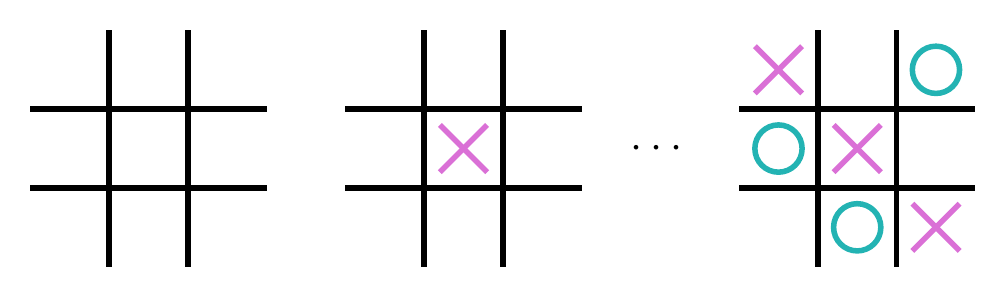
\begin{tikzpicture}
\begin{scope}
    % 画井字棋的网格
    \draw[line width=2] (0,1) -- (3,1);
    \draw[line width=2] (0,2) -- (3,2);
    \draw[line width=2] (1,0) -- (1,3);
    \draw[line width=2] (2,0) -- (2,3);
\end{scope}

\begin{scope}[xshift=4cm]
    % 画井字棋的网格
    \draw[line width=2] (0,1) -- (3,1);
    \draw[line width=2] (0,2) -- (3,2);
    \draw[line width=2] (1,0) -- (1,3);
    \draw[line width=2] (2,0) -- (2,3);
    
    % 画X(用交叉线表示)
    \draw[line width=2, Orchid] (1.2, 1.8) -- (1.8, 1.2); % 第二行中间 X
    \draw[line width=2, Orchid] (1.8, 1.8) -- (1.2, 1.2);
\end{scope}

\begin{scope}[xshift=6.5cm]
    \node[scale=1.5] at (1.5, 1.5) {$\cdots$};
\end{scope}

\begin{scope}[xshift=9cm]
    % 画井字棋的网格
    \draw[line width=2] (0,1) -- (3,1);
    \draw[line width=2] (0,2) -- (3,2);
    \draw[line width=2] (1,0) -- (1,3);
    \draw[line width=2] (2,0) -- (2,3);
    
    % 画X(用交叉线表示)
    \draw[line width=2, Orchid] (0.2, 2.8) -- (0.8, 2.2); % 第一行左侧 X
    \draw[line width=2, Orchid] (0.8, 2.8) -- (0.2, 2.2);
    
    \draw[line width=2, Orchid] (1.2, 1.8) -- (1.8, 1.2); % 第二行中间 X
    \draw[line width=2, Orchid] (1.8, 1.8) -- (1.2, 1.2);
    
    \draw[line width=2, Orchid] (2.2, 0.8) -- (2.8, 0.2); % 第三行右侧 X
    \draw[line width=2, Orchid] (2.8, 0.8) -- (2.2, 0.2);
    
    % 画O(用圆形表示)
    \draw[line width=2, TealBlue] (0.5, 1.5) circle(0.3); % 第二行左侧 O
    \draw[line width=2, TealBlue] (2.5, 2.5) circle(0.3); % 第一行右侧 O
    \draw[line width=2, TealBlue] (1.5, 0.5) circle(0.3); % 第三行中间 O
\end{scope}
\end{tikzpicture}

\end{document}
